\documentclass{beamer}
\usepackage[T1]{fontenc}
\usepackage[utf8]{inputenc}
\usepackage{graphicx}
\usepackage[normalem]{ulem}
\usepackage{xmpmulti}
% \usepackage[dvipsnames]{xcolor}

\newcommand{\emphh}[1]{\textcolor{blue}{\emph{#1}}}
\newcommand{\hilite}[1]{\emphh{#1}}
\title{Connected Dominating Sets in Triangulations}

\author{}
\author{%
  Prosenjit~Bose \and
  Vida~Dujmović \and
  Hussein~Houdrouge \and
  Pat~Morin \and
  Saeed~Odak}
\date{}

\setbeameroption{hide notes} % Only slides
%\setbeameroption{show only notes} % Only notes
% \setbeameroption{show notes on second screen=right} % Both


% \DeclareMathOperator{\tw}{tw}
% \DeclareMathOperator{\td}{td}
% \DeclareMathOperator{\wcol}{wcol}
% \DeclareMathOperator{\lvr}{\chi_{\ell-\mathrm{vr}}}
% \DeclareMathOperator{\pcn}{\chi_{p}}

\begin{document}

\begin{frame}
  % \begin{center}
    \maketitle
  % \end{center}
\end{frame}


\begin{frame}
  \frametitle{(Connected) Dominating Sets}

  \begin{itemize}
    \item $X\subseteq V(G)$ is a \emphh{dominating set} of $G$ if $N[X]=V(G)$
    \begin{center}
      \only<1>{\includegraphics[page=10]{figs/walkthrough}}%
      \only<2>{\includegraphics[page=11]{figs/walkthrough}}%
    \end{center}
    \item $X$ is \emphh{connected} if $G[X]$ is connected
  \end{itemize}
\end{frame}


\begin{frame}
  \frametitle{Connected Dominating Sets and Lush Spanning Trees}

  \begin{center}
    $X$ is a connected dominating set of $G$ \\[1em]
    $\Updownarrow$ \\[1em]
    $G$ has a spanning tree where vertices in $V(G)\setminus X$ are leaves.
    \only<1>{\includegraphics[page=11]{figs/walkthrough}}%
    \only<2>{\includegraphics[page=12]{figs/walkthrough}}%
    \only<3>{\includegraphics[page=9]{figs/walkthrough}}%
  \end{center}
\end{frame}

\begin{frame}
  \frametitle{Triangulations}

  \textbf{Theorem (Albertson, Berman, Hutchinson, and Thomassen 1990):}  Every triangulation has a \hilite{homemorphically irreducible} spanning tree.\\[2em]

  \uncover<2->{\textbf{Corollary:} Every $n$-vertex triangulation has a spanning tree with at least $n/2$ leaves.\\[2em]}

  \uncover<3->{\textbf{Corollary:} Every $n$-vertex triangulation has a connected dominating set of size at least $n/2$.}

\end{frame}

\begin{frame}
  \frametitle{Induced Outerplanar Graphs}

  \textbf{Theorem (Angelini, Evans, Frati, and Gudmundsson 2016):}  Every $n$-vertex triangulation $G$ has an induced outerplane graph $G[Y]$ with at least $n/2$ vertices.
  \begin{center}
    \only<1>{\includegraphics[page=13]{figs/walkthrough}}%
    \only<2->{\includegraphics[page=14]{figs/walkthrough}}%
  \end{center}

  \uncover<2->{Gives a bound of $n/2$ for the \emphh{SEFENOMAP} graph drawing problem.\\[1em]}
  \uncover<3->{\textbf{Observation:} If $X$ is a connected dominating set then $G-X$ is an induced outerplace graph with $n-|X|$ vertices.}
\end{frame}

\begin{frame}
  \frametitle{The Benchmark: $n/3$}

  \begin{center}
    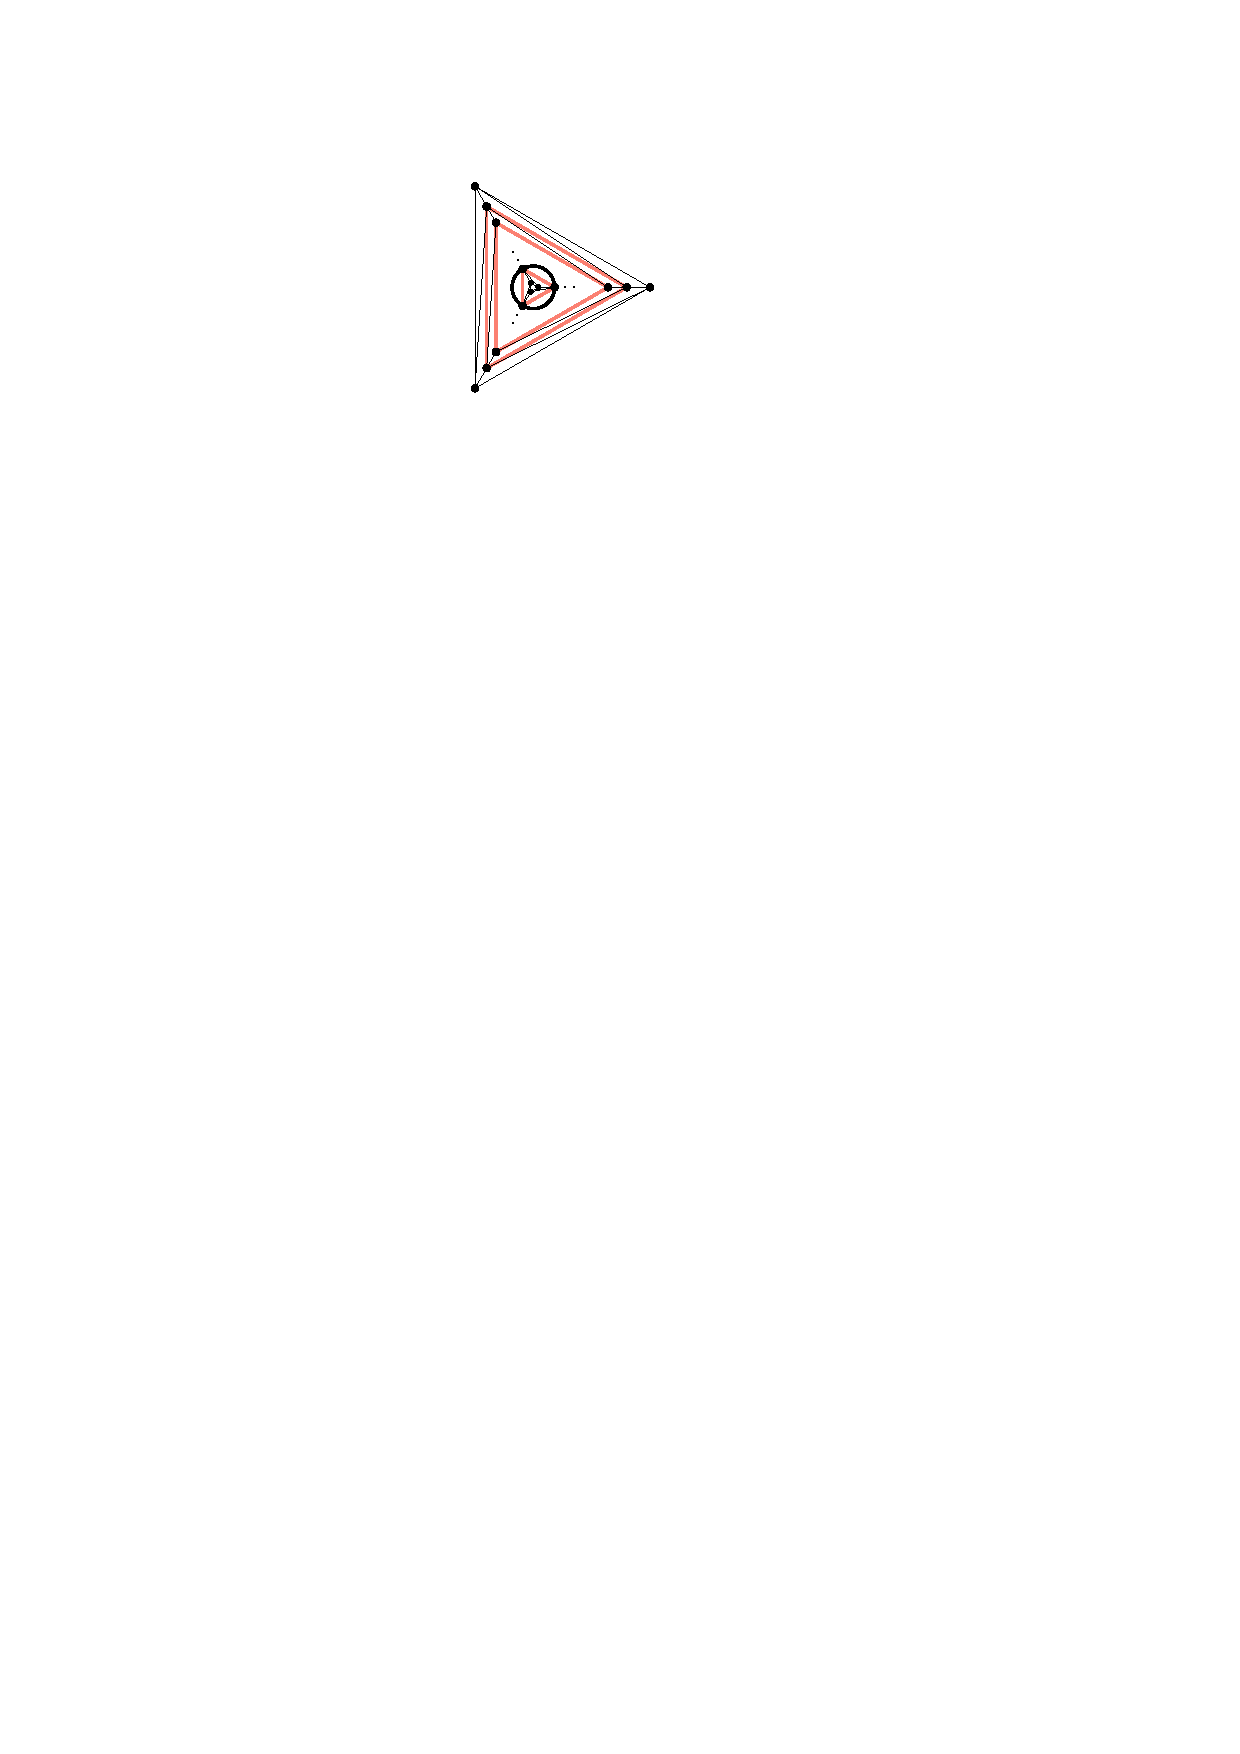
\includegraphics[height=.7\textheight]{figs/nover3}
  \end{center}
\end{frame}


\begin{frame}
  \frametitle{Main Result}

  \textbf{Theorem:}  Every $n$-vertex triangulation $G$ has a connected dominating set of size at most $10n/21=\overline{0.476190}n$.\\[2em]

  \textbf{Corollary:}  Every $n$-vertex triangulation $G$ has a spanning tree with at least $11n/21=\overline{0.523809}n$ leaves.\\[2em]

  \textbf{Corollary:}  Every $n$-vertex triangulation $G$ has an induced outerplane graph $G[Y]$ with at least $11n/21=\overline{0.523809}n$ vertices.\\[2em]

  Gives a bound of $11n/21$ for the SEFENOMAP problem.
\end{frame}

\begin{frame}
  \frametitle{Greedy Strategy}

  \begin{tabular}{p{.6\textwidth}c}

    $\textsc{NaïveGreedy}(G)$:\newline
    $X\gets\{v_0\}$ \newline
    Repeat until $N[X]=V(G)$: \newline
    --- Let $v\in N(X)$ maximize $|N(v)\setminus N(X)|$ \newline
    --- Set $X\gets X\cup\{v\}$
    &
    \raisebox{-\height}{%
      \only<1>{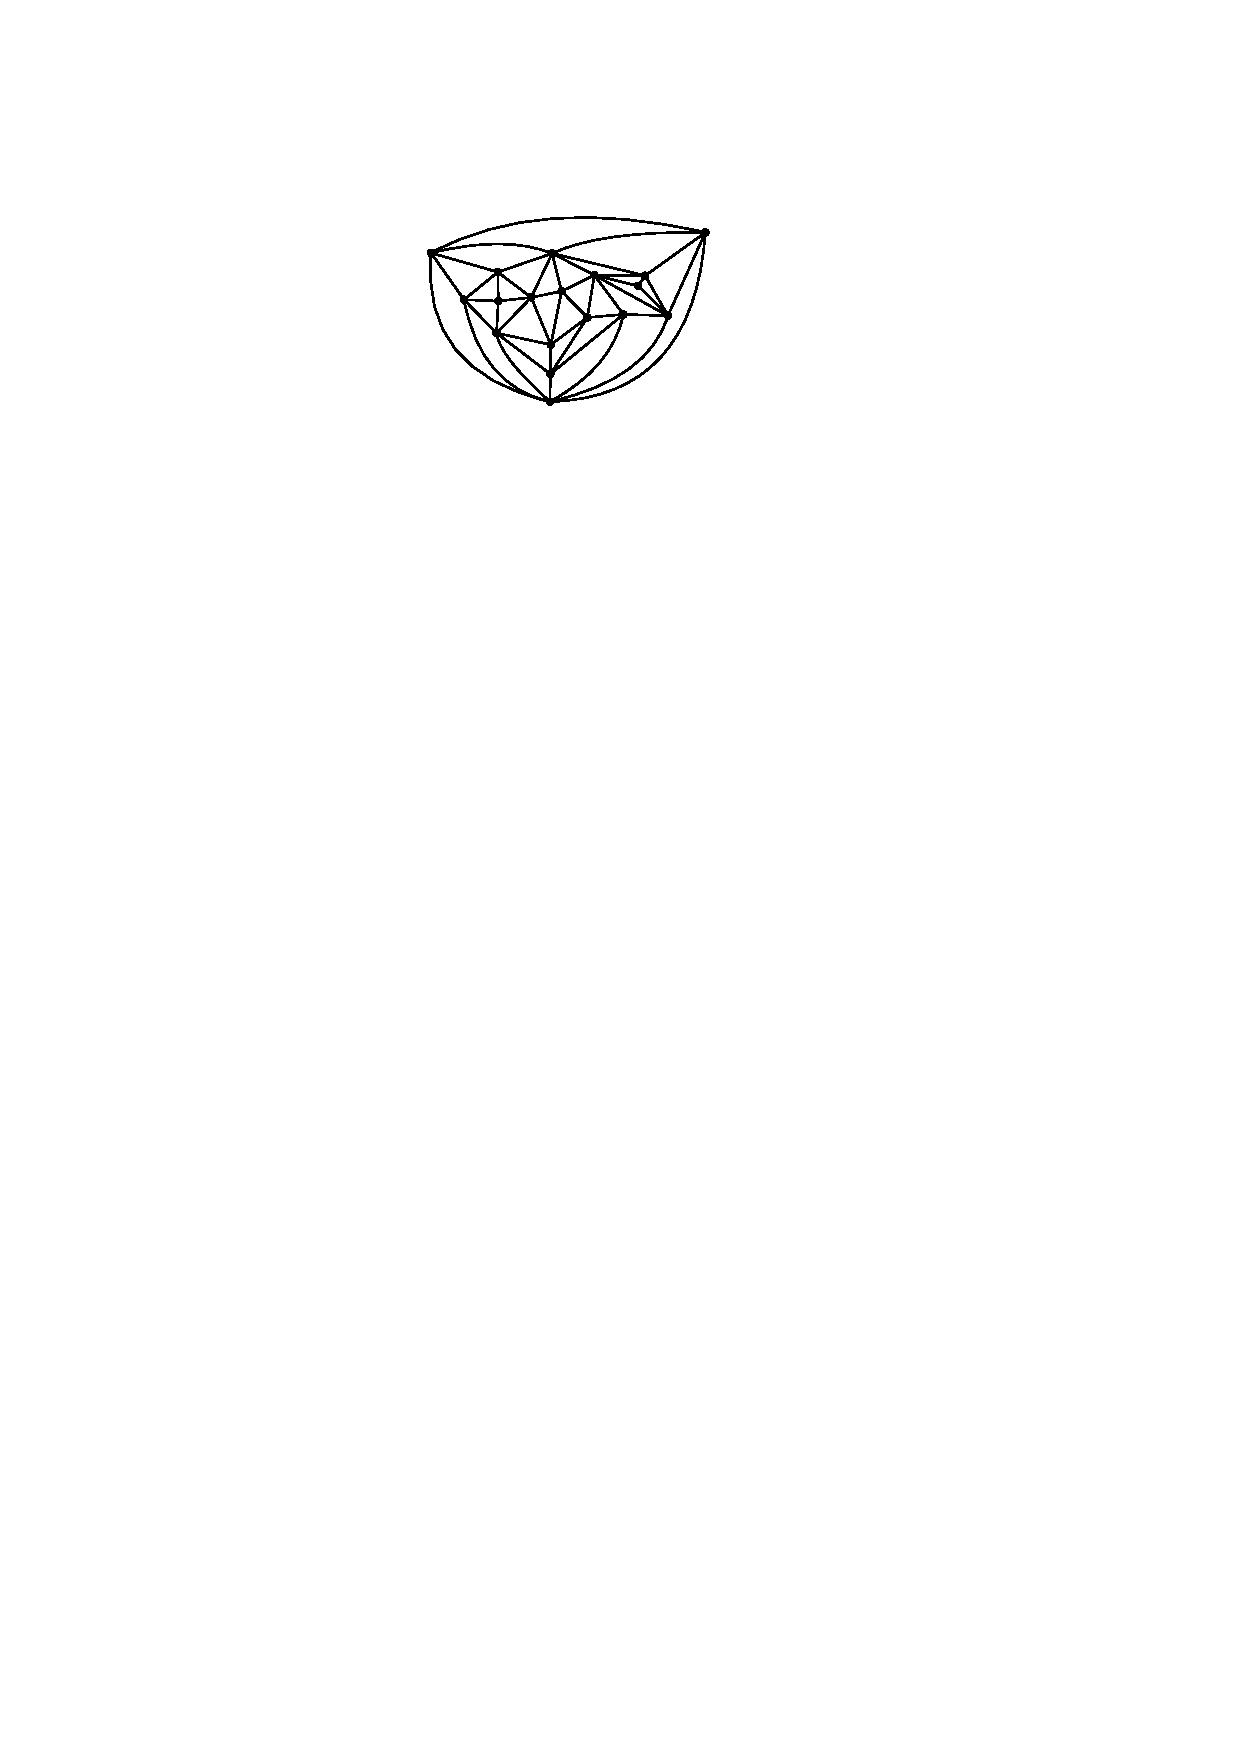
\includegraphics[width=.4\textwidth,page=1]{figs/walkthrough}}%
      \only<2>{\includegraphics[width=.4\textwidth,page=2]{figs/walkthrough}}%
      \only<3>{\includegraphics[width=.4\textwidth,page=3]{figs/walkthrough}}%
      \only<4>{\includegraphics[width=.4\textwidth,page=4]{figs/walkthrough}}%
      \only<5>{\includegraphics[width=.4\textwidth,page=5]{figs/walkthrough}}%
      \only<6-7>{\includegraphics[width=.4\textwidth,page=6]{figs/walkthrough}}%
      \only<8>{\includegraphics[width=.4\textwidth,page=7]{figs/walkthrough}}%
      \only<9>{\includegraphics[width=.4\textwidth,page=8]{figs/walkthrough}}%
      % \only<10>{\includegraphics[width=.4\textwidth,page=9]{figs/walkthrough}}%
    }
  \end{tabular}


  \begin{tabular}{p{.6\textwidth}c}
    \raggedright
    \uncover<4->{
    \textbf{Ideally:} $|N(v)\setminus N(X)|\ge c$ at each step \newline
    Would give $|X|\le n/c$\vspace{1em}
    }

    \uncover<6->{
    \textbf{Problem:} Impossible to guarantee $|N(v)\setminus N(X)|\ge 2$.\vspace{1em}
    }

    & \uncover<7->{\raisebox{-\height}{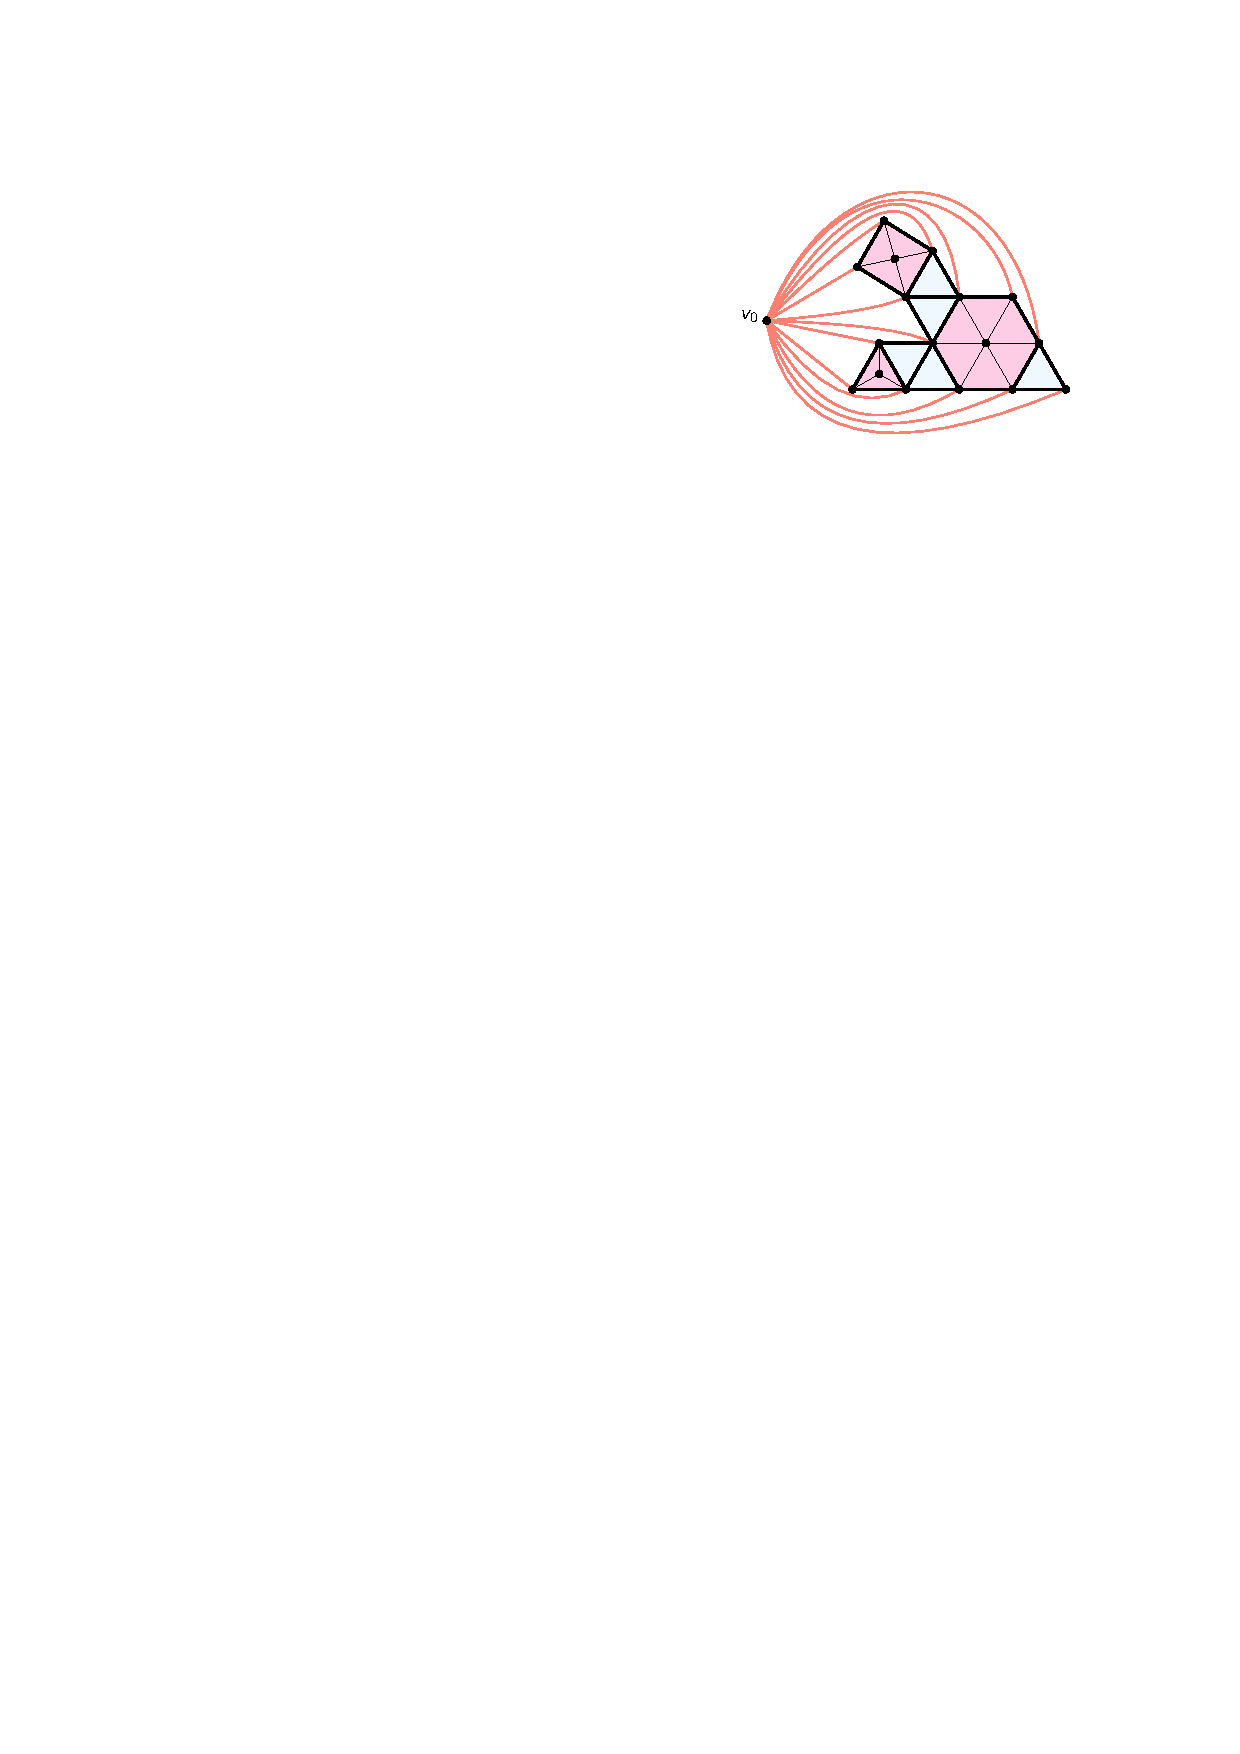
\includegraphics[width=.4\textwidth]{figs/noguarantee}}}
  \end{tabular}
\end{frame}


\begin{frame}
  \frametitle{$1$-Critical Graphs}

  All inner faces are triangles \newline
  All vertices have inner degree $\le 1$ \\[3em]

  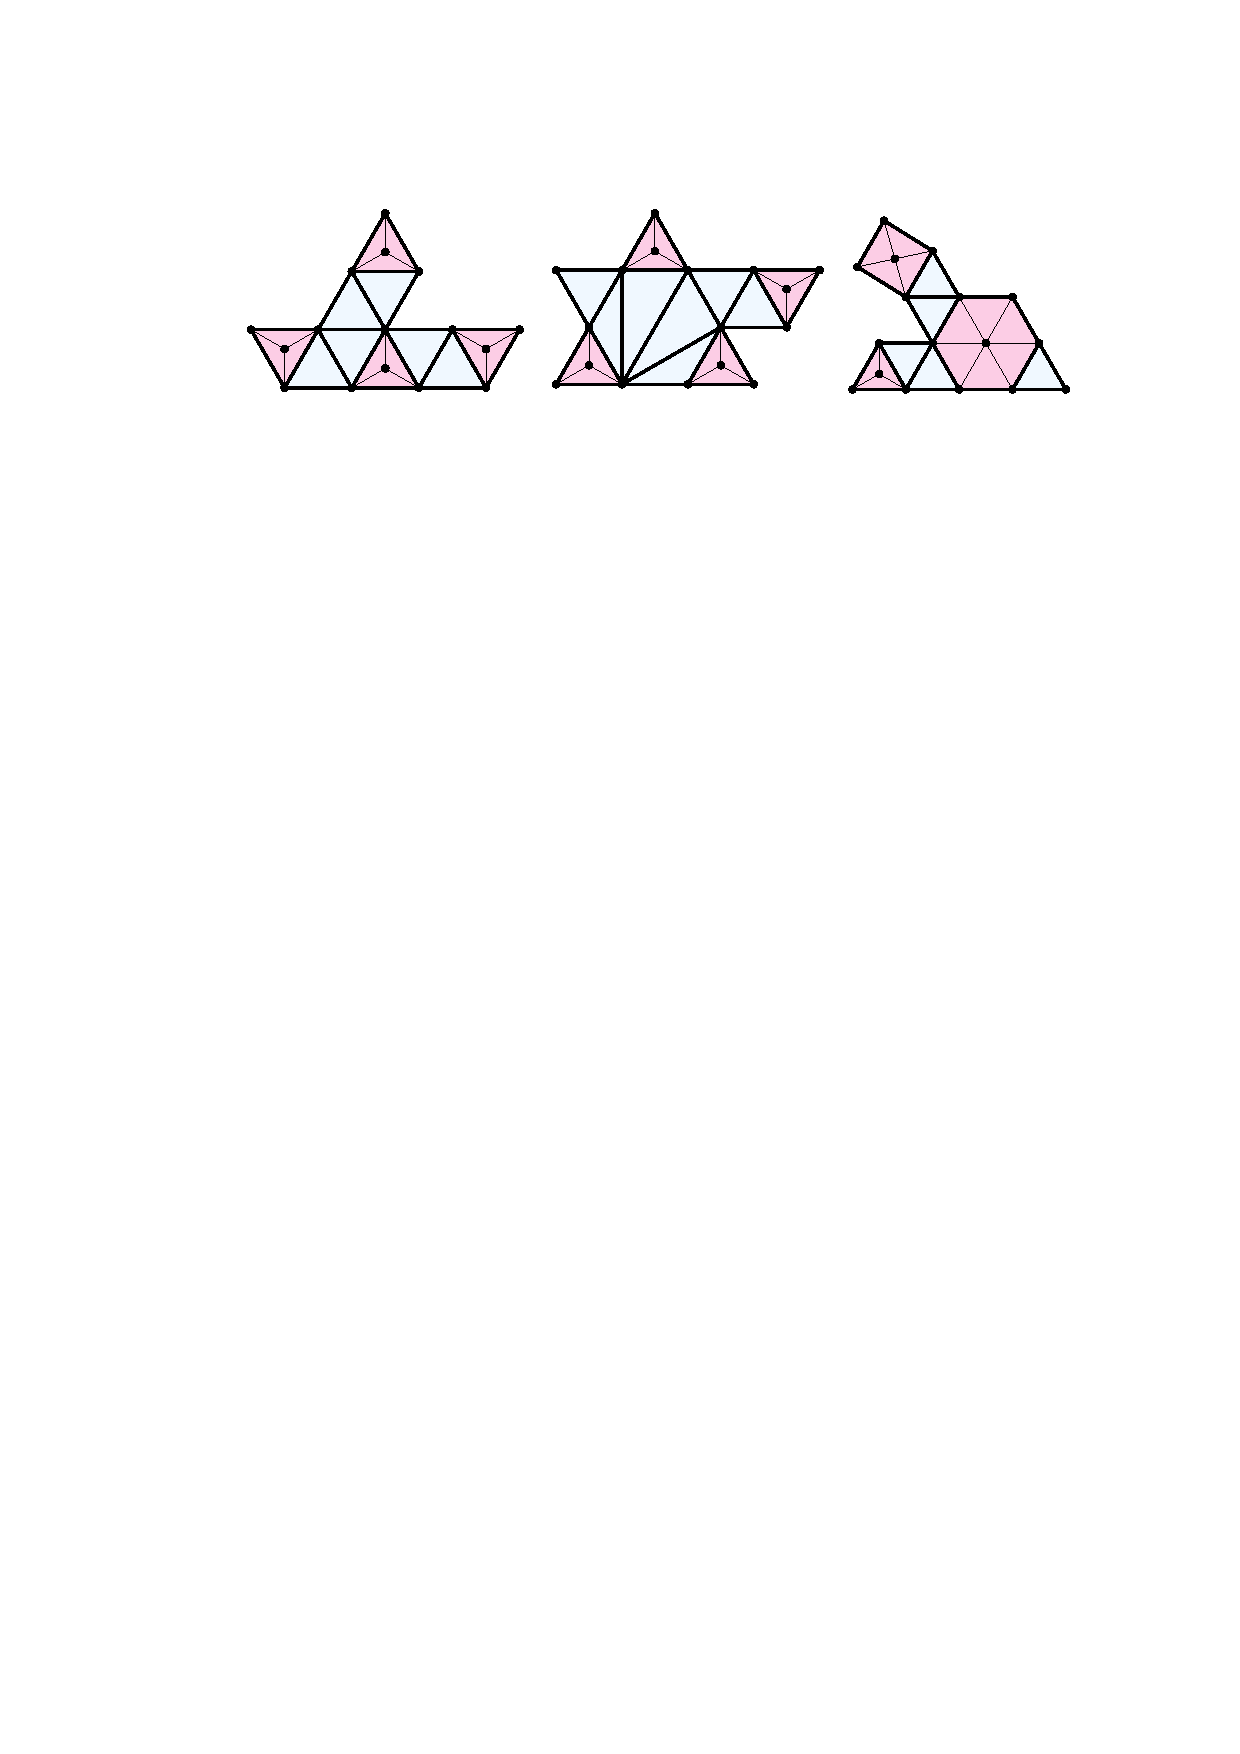
\includegraphics[width=.98\textwidth]{figs/critical}\\[3em]

  \textbf{Lemma:} $\text{\#inner vertices} \le \tfrac{1}{4}\text{\#vertices}$
\end{frame}

\begin{frame}
  \frametitle{A First Attempt}

  \textbf{Theorem:} $\textsc{NaïveGreedy}(G)$ produces a dominating set of size at most $4n/7$.

  \uncover<2->{
  \textit{Proof:} Takes vertices of inner-degree at least $2$ until $G-X$ is $1$-critical.
  \begin{center}
    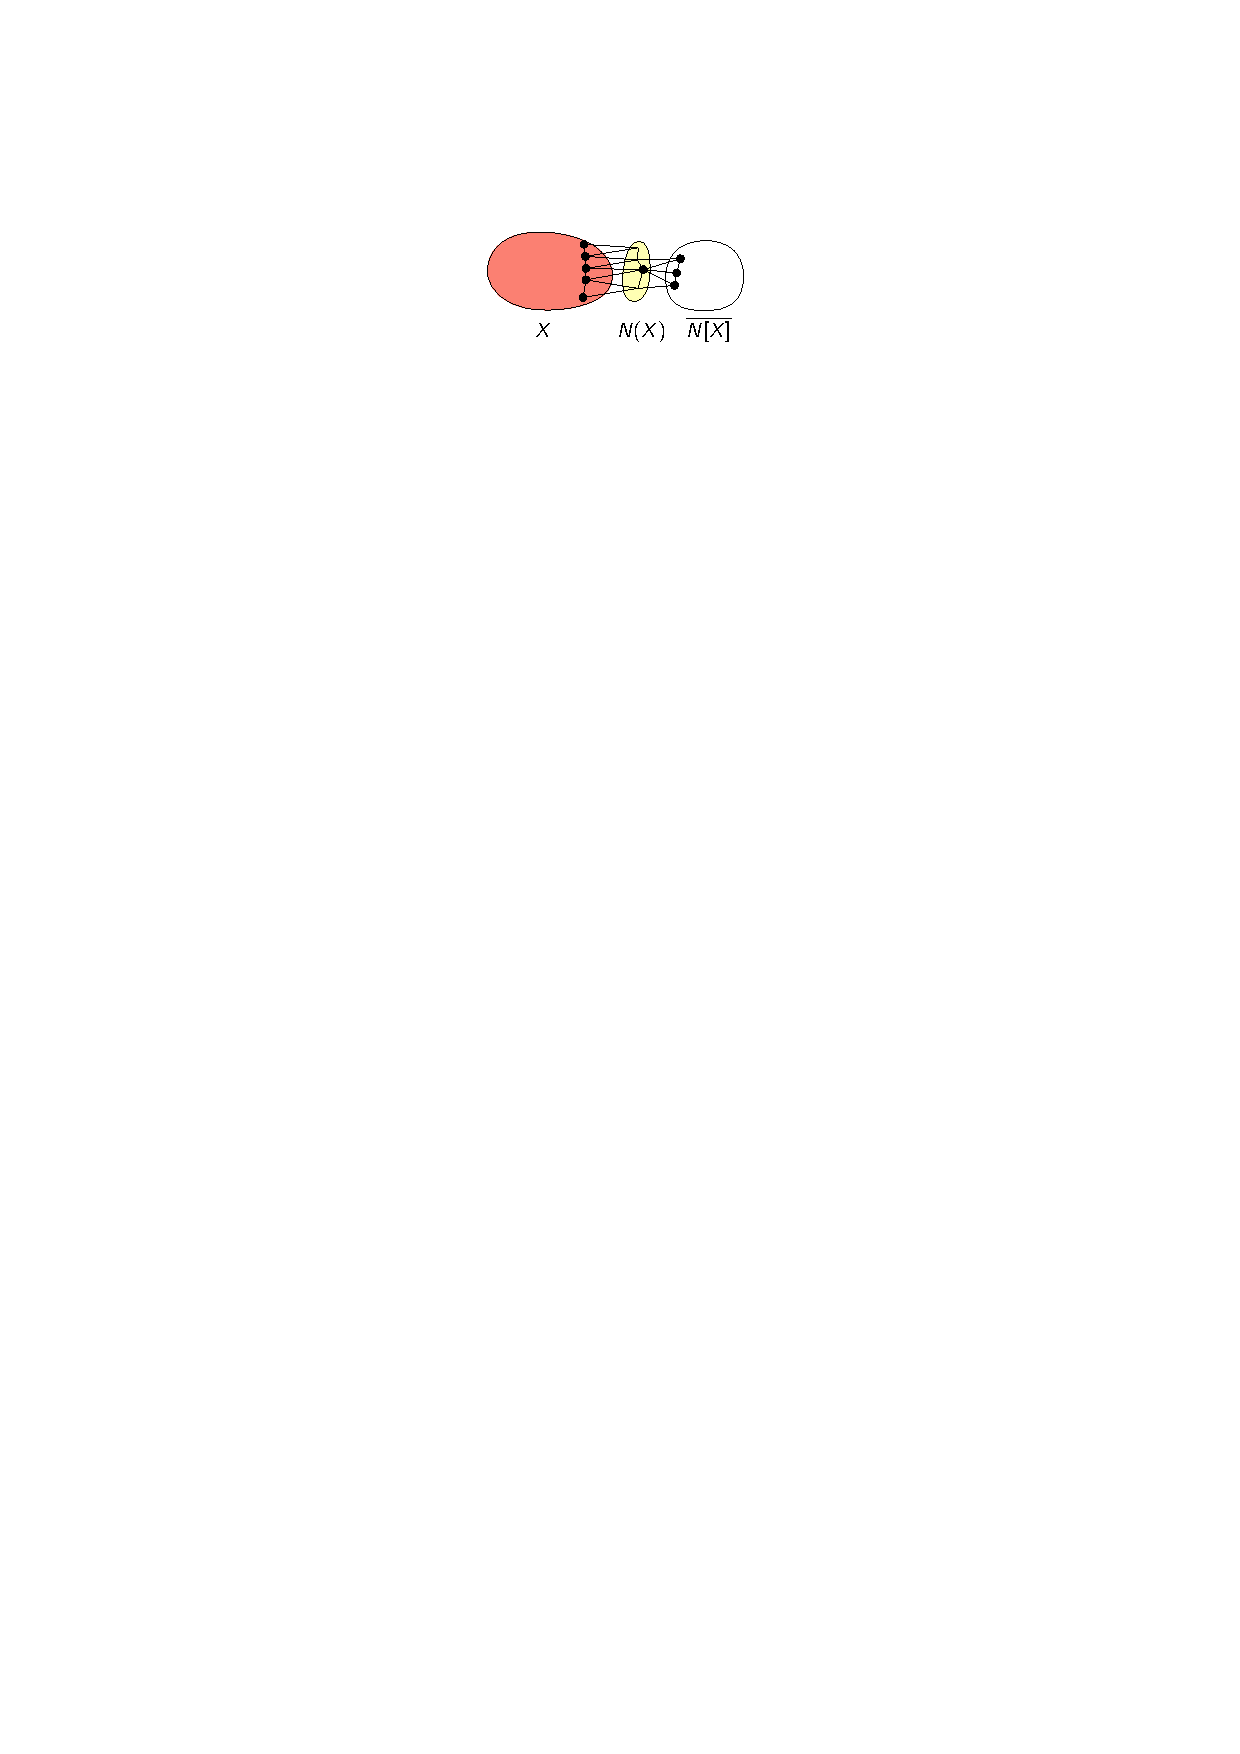
\includegraphics{figs/greedy} \includegraphics[page=6]{figs/walkthrough}
  \end{center}
  \[
     |X| = r + I , \quad 2r + I \le n, \quad I \le (n-r)/4
  \]
  Maximized when $r=3n/7$, $I=n/7$
  }
\end{frame}


\begin{frame}
  \frametitle{Lesson}

  To beat $n/2$, we need to choose vertices of inner-degree at least $3$
\end{frame}

\end{document}

\begin{frame}
  \frametitle{The Strong Graph Product $\boxtimes$}

  \includegraphics[page=1]{figs/blowup}
  % \only<2>{\includegraphics[page=2]{figs/blowup}}
  % \only<3>{\includegraphics[page=3]{figs/blowup}}
  % \includegraphics{figs/product-lhs} \raisebox{.11\textwidth}{$=$}
  % \includegraphics{figs/product-rhs}%
\end{frame}

\begin{frame}
  \frametitle{Motivation: Graph Product Structure Theory}

  \only<1>{\includegraphics[page=1]{figs/procedure}}%
  \only<2>{\includegraphics[page=2]{figs/procedure}}%
  \only<3->{\includegraphics[page=3]{figs/procedure}}

  To solve some problem on $G$:
  \begin{itemize}
    \item<2->Show $G\subseteq H\boxtimes K_c$ where $c$ and $\tw(H)$ are small
    \item<3->Show $H$ has solution of ``cost'' at most $f(\tw(H))$
    \item<3->Extend to solution of $H\boxtimes K_c$ of ``cost'' $f(\tw(H))\cdot c$
  \end{itemize}
  % \textbf{Theorem (Dujmović, Joret, Micek, M., Ueckerdt, Wood 2019):} For every planar graph $G$ there exists
  % \begin{itemize}
  %   \item a graph ${\color{red}H}$ of treewidth at most $3$; and
  %   \item a path ${\color{blue}P}$; such that
  % \end{itemize}
  % $G$ is isomorphic to a subgraph of ${\color{red}H}\boxtimes {\color{blue}P\boxtimes K_3}$\newline ($G\subseteq {\color{red}H}\boxtimes {\color{blue}P\boxtimes K_3}$).\vspace{1em}
  %
  % \includegraphics[scale=.6]{figs/planar-subgraph}%
  % \only<2>{\raisebox{.066\textwidth}{$\subseteq$}\includegraphics[scale=.6]{figs/product-rhs}}%
  % \only<3>{\raisebox{.066\textwidth}{$\subseteq$}\includegraphics[scale=.6]{figs/product-lhs}}
  %
  % \uncover<4->{
  %   Applications:
  %   \begin{itemize}
  %     \item For monotone $\rho$, $\rho(G)\le \rho({\color{red}H}\boxtimes {\color{blue}K_c})$
  %     \item For many $\rho$, $\rho(H\boxtimes P)\le {\color{red}f(\tw(H))}\cdot {\color{blue}c}$
  %   \end{itemize}
  %
  % }
  % \note[item]{State theorems}
  % \note[item]{Used to bound many graph parameters for planar graphs}
  % \note[item]{Similar theorems hold for some other graph families}
  % \note[item]{Usually parameter is bounded by a fast growing function of $\tw(H)$ and the $P\boxtimes K_3$ factor increases the bound by a constant factor.}
  % \note[item]{In other applications, $\tw(H)$ appears as a factor in some function of $n$, for example, $tw(H)\log\log n$}
  % \note[item]{In one application, $\tw(H)$ affects the asymptotic growth, for example $\log n/log^{(\tw(H))} n$}
  % \note[item]{Example, non-repetitive chromatic number is at most $4^{\tw(H)}\cdot 12$}
\end{frame}

\begin{frame}
  \frametitle{The Graph Minor Relation $\preceq$}

  \begin{center}
    \begin{tabular}{ccc}
      \includegraphics[page=1]{figs/minors} & &
      \includegraphics[page=2]{figs/minors} \\
      $K_4$ & $\preceq$ & $G$
    \end{tabular}
  \end{center}
  \only<2->{$G$ is \emph{$X$-minor-free} if $X \not\preceq G$}
\end{frame}


\begin{frame}
  \frametitle{The Grid-Minor Theorem}

  \uncover<1->{\textbf{Theorem (Robertson-Seymour 1986):}  For any planar graph $X$, every $X$-minor-free graph $G$ satisfies $\tw(G)\le f(X)$.\vspace{1em}}

  \uncover<3>{\textbf{Theorem (Robertson-Seymour 1986):}  Every $k$-vertex planar graph $X$ is a minor of the $2k\times 2k$ grid.

  \textbf{Theorem (Chuzoy and Tan 2019):} Every graph of treewidth at least $ck^{9+\epsilon}$ contains a $2k\times 2k$ grid minor.\vspace{1em}}

  \uncover<2->{\textbf{Corollary (RSCT):} For any planar graph $X$ every $X$-minor-free graph $G$ satisfies $\tw(G)\le c|V(X)|^{9+\epsilon}$.\vspace{1em}}

  % \uncover<4->{Can we refine RS86 to get $G\subseteq H\boxtimes K_c$ where $\tw(H)$ depends on the ``complexity'' of $X$?}

  \note[item]{Note that the treewidth of $G$ depends on the size of $X$}
  \note[item]{Can it depend, instead, on the complexity of $X$?}
  \note[item]{Not really, the $k\times k$ grid excludes an $\Omega(k)$ vertex star as a minor.}
\end{frame}

\begin{frame}
  \frametitle{The Grid-Minor Theorem}

  \textbf{Corollary (RSCT):} For any planar graph $X$ every $X$-minor-free graph $G$ satisfies $\tw(G)\le c|V(X)|^{9+\epsilon}$.\vspace{1.5em}

  \uncover<2->{Q: Can we bound $\tw(G)$ by the ``complexity'' of $X$?\vspace{.5em}}

  \uncover<3->{\raisebox{8ex}{A: No}\hspace{2em} \includegraphics{figs/star-vs-grid}}

  \uncover<4->{Q:Can we refine RS86 to get $G\subseteq H\boxtimes K_c$ where $\tw(H)$ depends on the ``complexity'' of $X$ and only $c$ depends on $|V(X)|$?\vspace{.5em}}

  % \uncover<5->{A: Maybe, since $\boxplus_{k\times k}\subseteq K_1\boxtimes K_{k^2}$}
\end{frame}


\begin{frame}
  \frametitle{Treedepth}
  \framesubtitle{The right measure of complexity for $X$}

  \centering{\includegraphics{figs/treedepth}}

  \[  \td(X) = \min\{\operatorname{height}(T): \
    \mbox{$T$ is a tree and $X\subseteq \operatorname{closure}(T)$} \} \]

  \begin{itemize}
    \item<2-> $\td(T) \le \operatorname{height}(T)$ for any tree $T$
    \item<3-> $\td(K_c\oplus I_n) = c+1$
  \end{itemize}
\end{frame}


\begin{frame}
  \frametitle{Theorem 1}

  \uncover<1-3>{\textbf{Theorem (Robertson-Seymour 1986):}  For any planar graph $X$, every $X$-minor-free graph $G$ satisfies $\tw(G)\le f(X)$.\vspace{1em}}

  \uncover<2->{\textbf{Corollary (RSCT):} For any planar graph $X$ every $X$-minor-free graph $G$ satisfies $\tw(G)\le c|V(X)|^{9+\epsilon}$.\vspace{1em}}

  \uncover<3->{\textbf{Theorem 1:}  For any planar graph $X$, every $X$-minor-free graph $G$ satisfies $G\subseteq H\boxtimes K_{c}$ where $\tw(H)\le 2^{\td(X)+1}$ and $c=c(X)$.}
\end{frame}


\begin{frame}
  \frametitle{Application: Weak Colouring Numbers}

  \textbf{Theorem 1:}  For any planar graph $X$, every $X$-minor-free graph $G$ satisfies $G\subseteq H\boxtimes K_{c}$ where $\tw(H)\le 2^{\td(X)+1}$ and $c=c(X)$.\vspace{1em}

  \begin{center}
    \includegraphics{figs/rweak}
  \end{center}

  \textbf{Application 1:} For any planar graph $X$, any $r\ge 1$, and any $X$-minor-free graph $G$, the $r$-th weak colouring number of $G$ satisfies
  \[  \wcol_r(G) \le r^{f(\td(X))}\cdot c(X) \enspace . \]
\end{frame}

\begin{frame}
  \frametitle{Application: $p$-Centered Colouring}

  \textbf{Theorem 1:}  For any planar graph $X$, every $X$-minor-free graph $G$ satisfies $G\subseteq H\boxtimes K_{c}$ where $\tw(H)\le 2^{\td(X)+1}$ and $c=c(X)$.\vspace{1em}

  \begin{center}
    \includegraphics{figs/pcentered}
  \end{center}

  (Pilipczuk-Siebertz 2021)

  \textbf{Application 2:} For any planar graph $X$, any $p\ge 1$, and any $X$-minor-free graph $G$, the $p$-centered chromatic number of $G$ is at most
  \[  \chi_p(G) \le p^{f(\td(X))}\cdot c(X) \enspace . \]
\end{frame}

\begin{frame}
  \frametitle{Application: Adjacency Labelling}

  \textbf{Theorem 1:}  For any planar graph $X$, every $X$-minor-free graph $G$ satisfies $G\subseteq H\boxtimes K_{c}$ where $\tw(H)\le 2^{\td(X)+1}$ and $c=c(X)$.\vspace{1em}

  \begin{center}
    \includegraphics[page=4,scale=.7]{figs/labelling-scheme}
  \end{center}

  (Gavoille et al.) \\
  \textbf{Application 3:} For any planar graph $X$, any $p\ge 1$, and any $X$-minor-free $n$-vertex graph $G$, there exists an adjacency labelling scheme for $G$ in which labels have length at most
  \[   \log n + f(\td(X))\log\log n + c(X) \enspace . \]
\end{frame}


\begin{frame}
  \frametitle{Application: $\ell$-Vertex-Ranking}

  \textbf{Theorem 1:}  For any planar graph $X$, every $X$-minor-free graph $G$ satisfies $G\subseteq H\boxtimes K_{c}$ where $\tw(H)\le 2^{\td(X)+1}$ and $c=c(X)$.\vspace{1em}

  \begin{center}
    \includegraphics{figs/lvr}
  \end{center}

  (Bose, Dujmović, Javarsineh, M. 2020)
  \textbf{Application 4:} For any planar graph $X$, any $\ell\ge 2$, and any $X$-minor-free $n$-vertex graph $G$, the $\ell$-vertex-ranking number of $G$ satisfies
  \[  \chi_{\ell\mathrm{-vr}}(G) \le \frac{\log n}{\log^{(f(\td(X)))} n}\cdot c(\ell,X) \enspace . \]
\end{frame}


%%%%%%%%%%%%%%%%%%%%%%%%%%%%%%%%%%%%%%%%%%%%%%%%%%%%%%%%%%%%%%%%%%%%%%%%%
\begin{frame}
  \frametitle{The General Result}

  \textbf{Theorem 1:}  For any planar graph $X$, every $X$-minor-free graph $G$ satisfies $G\subseteq H\boxtimes K_{c}$ where $\tw(H)\le 2^{\td(X)+1}$ and $c=c(X)$.\vspace{1em}

  \textbf{Theorem 2:}  For any graph $X$, every $X$-minor-free graph $G$ satisfies $G\subseteq H\boxtimes K_{ct}$ where $\tw(H)\le 2^{\td(X)+1}$, $c=c(X)$, and $t=\tw(G)$.\vspace{1em}

\end{frame}


%%%%%%%%%%%%%%%%%%%%%%%%%%%%%%%%%%%%%%%%%%%%%%%%%%%%%%%%%%%%%%%%%%%%%%%%%
\begin{frame}
  \frametitle{Proof Ideas}
  \framesubtitle{$H$-Partitions}

  \textbf{Theorem 2:}  For any graph $X$, every $X$-minor-free graph $G$ has an $H$-partition $(B_x:x\in V(H))$ where $\tw(H)\le 2^{\td(X)+1}$ and $|B_x|\le c(X)\cdot\tw(G)$ for each $x\in V(H)$.\vspace{1em}

  \includegraphics[page=4]{figs/procedure}%

  $vw\in E(G)$, $v\in B_x$, $w\in B_y$ $\Rightarrow$ $x=y$ or $xy\in E(H)$
\end{frame}

%%%%%%%%%%%%%%%%%%%%%%%%%%%%%%%%%%%%%%%%%%%%%%%%%%%%%%%%%%%%%%%%%%%%%%%%%
\begin{frame}
  \frametitle{Proof Ideas}
  \framesubtitle{Universal treewidth-$h$ graph}

  Instead of $X$, assume $G$ is $U_{h,d}$-minor-free, where $h=\td(X)$ and $d=|V(X)|$.

  \begin{center}
    \only<1>{\includegraphics{figs/uhd.pdf}}%
    \only<2->{\includegraphics[page=2]{figs/uhd.pdf}}%
  \end{center}

  \only<2->{Inductively, we even assume $(K_k\oplus U_{h,d})$-minor-free}
  % \includegraphics[page=4]{figs/procedure}%
\end{frame}

%%%%%%%%%%%%%%%%%%%%%%%%%%%%%%%%%%%%%%%%%%%%%%%%%%%%%%%%%%%%%%%%%%%%%%%%%
\begin{frame}
  \frametitle{Proof Ideas}
  \framesubtitle{Rooted Minors}

  Assume $G$ has no $R$-rooted $K_k\oplus U_{h,d}$ minor, use decomposition similar to Kawarabayashi (2004).

  \begin{center}
    \includegraphics[scale=0.6]{../figs/c-subgraph1.pdf}
  \end{center}



  % \includegraphics[page=4]{figs/procedure}%
\end{frame}


%%%%%%%%%%%%%%%%%%%%%%%%%%%%%%%%%%%%%%%%%%%%%%%%%%%%%%%%%%%%%%%%%%%%%%%%%
\begin{frame}
  \frametitle{Proof Ideas}
  \framesubtitle{Erd\H{o}s-Posa}

  Hit all $R$-rooted copies of $K_{k+d}\oplus U_{h-1,d}$ in $C^0$ with a small set $X$
  \begin{center}
    \includegraphics[scale=0.6]{../figs/combining-minors4.pdf}
  \end{center}

  % \includegraphics[page=4]{figs/procedure}%
\end{frame}


%%%%%%%%%%%%%%%%%%%%%%%%%%%%%%%%%%%%%%%%%%%%%%%%%%%%%%%%%%%%%%%%%%%%%%%%%
\begin{frame}
  \frametitle{Proof Ideas}
  \framesubtitle{Divide and Conquer}

  \begin{center}
    \includegraphics[scale=.66]{../figs/final-clique-sums1.pdf}
  \end{center}

  $C_0-X$ is $K_{k+d}\oplus U_{h-1,d}$-minor free.

  $C_1,\ldots,C_r$ are smaller and $K_{k}\oplus U_{h,d}$-minor-free.

  % \includegraphics[page=4]{figs/procedure}%
\end{frame}

\begin{frame}
  \frametitle{Weak Colouring Numbers}

  \textbf{Application 1:} For any planar graph $X$, any $r\ge 1$, and any $X$-minor-free graph $G$, the $r$-th weak colouring number of $G$ satisfies
  \[  \wcol_r(G) \le r^{f(\td(X))}\cdot c(X) \enspace . \]

  \textbf{Theorem:} For any graph $X$, any $r\ge 1$, and any $X$-minor-free graph $G$, the $r$-th weak colouring number of $G$ satisfies
  \[  \wcol_r(G) \le r^{f(\td(X))}\cdot c(X) \enspace . \]
\end{frame}



\begin{frame}
  \frametitle{Extension to Apex-Minor-Free Graphs}

  \textbf{Theorem 1:}  For any planar graph $X$, every $X$-minor-free graph $G$ satisfies $G\subseteq H\boxtimes K_{c}$ where $\tw(H)\le 2^{\td(X)+1}$ and $c=c(X)$.\vspace{1em}

  \textbf{Theorem 3:}  For any \emph{apex} graph $X$, every $X$-minor-free graph $G$ satisfies $G\subseteq H\boxtimes P\boxtimes K_{c}$ where $\tw(H)\le 2^{\td(X)+1}$ and $c=c(X)$.\vspace{1em}
\end{frame}


\begin{frame}
  \frametitle{Summary}


  \textbf{Main Result:}  For any planar graph $X$, every $X$-minor-free graph $G$ satisfies $G\subseteq H\boxtimes K_{c}$ where $\tw(H)\le 2^{\td(X)+1}$ and $c=c(X)$.\vspace{1em}

  \uncover<2->{\textbf{Open Question:} Improve the dependence on $\td(X)$}\vspace{1em}

  \uncover<3->{\textbf{Open Question:} For any graph $X$, every $X$-minor-free graph $G$ satisfies $G\subseteq H\boxtimes K_{ct}$ where $\tw(H)\le f(\td(X))$, $c=c(X)$, and $t=\tw(G)$.\vspace{1em}
  }

  \begin{center}
    \uncover<4->{\Huge Thank You!}
  \end{center}
\end{frame}

% \begin{frame}
%   \frametitle{Main Theorem}
%
%   \textbf{Theorem 1:}  For any planar graph $X$, every $X$-minor-free graph $G$ satisfies $G\subseteq H\boxtimes K_{c\tw(X)}$ where $\tw(H)\le 2^{\td(X)+1}$.
%
%   \uncover<3->{\textbf{Theorem (Robertson-Seymour 1986):}  Every $k$-vertex planar graph $X$ is a minor of the $2k\times 2k$ grid.
%
%   \textbf{Theorem (Chuzoy and Tan 2019):} Every graph of treewidth at least $ck^9+\epsilon$ contains a $2k\times 2k$ grid minor.\vspace{1em}}
%
%   \uncover<2->{\textbf{Corollary (RSCT):} For any planar graph $X$ every $X$-minor-free graph $G$ satisfies $\tw(G)\le c|V(X)|^{9+\epsilon}$.}
% \end{frame}



\end{document}
